%% This is an example first chapter.  You should put chapter/appendix that you
%% write into a separate file, and add a line \include{yourfilename} to
%% main.tex, where `yourfilename.tex' is the name of the chapter/appendix file.
%% You can process specific files by typing their names in at the
%% \files=
%% prompt when you run the file main.tex through LaTeX.
\section{Graphs and intersections}
\label{sec:graphs}


\subsection{Graphs}

A graph $G$ is defined as $G = (V,E)$, where $V$ is the set of vertices and $E$ the set of
edges, where $E \subseteq \binom{V}{2}$. The vertices $v,w \in V$ such that $e = vw \in E$
links are called the \textit{endpoints} of $e$.

\begin{defn}
  An embedding of a graph $G$ into a surface $\Sigma$ is a mapping of $G$ in
  $\Sigma$ where the vertices correspond to distinct points and the edges
  correspond to simple arcs connecting the images of their endpoints.
  \cite{goyalGraphEmbeddingTechniques2017}.
\end{defn}

A graph $G$ is planar if there is an embedding of this graph that does not have
any crossing between the edges.

\begin{defn}
  Let $G = (V,E)$ and $S \subset V$, an induced subgraph is a graph $H$ of $G$ whose
  vertex set is $S$ and its edge set $F = \{vw : v,w \in S, vw \in E\}$.
\end{defn}

\begin{defn}
  Let $G = (V,E)$ its complement graph $\overline{G}$ is the graph such that its edge set
  is defined as: $\{vw: v,w\in V, vw\notin E\}$.
\end{defn}

\begin{defn}
  $H$ is called a \textit{minor} of $G$ if $H$ can be constructed by deleting edges and vertices,
  or contracting edges.
\end{defn}

\begin{theorem}[Kuratowski]
  A graph $G$ is planar if and only if it does not contain $K_5$ or $K_{3,3}$ as a minor or
  a induced subgraph.
\end{theorem}

\begin{defn}
  A path $P_n$ in a graph $G$ is a sequence of vertices $v_1v_2v_3\dots v_n$ such
  that $v_iv_{i+1} \in E$.
\end{defn}

\begin{defn}
  A cycle $C_n$ in a graph $G = (V,E)$ is a path $v_1\dots v_n$ such that $v_1 = v_n$.
\end{defn}

\begin{defn}
  A chord of a cycle $C_n$ with $n \geq 4 $ is an edge that connects two non consecutive vertices
  of $C_n$.
\end{defn}

\begin{defn}
  A triangular chord of a cycle is a chord that will create a new triangle ($C_3$).
\end{defn}


\begin{defn}
  A graph $G = (V,E)$ is complete if every pair of distinct $v_1,v_2 \in V$ are
  adjacent. This is denoted $K_n$ with $n$ the size of the graph. If $G$ is an
  induced graph of $H$ then $G$ is a clique of $H$.
\end{defn}

\begin{defn}
  A graph $G$ is bipartite if there exist two disjoint subsets $A,B \subset V$ such
  that $A\cup B = V$ and each edge $e\in E$ has an endpoint on $A$ and the
  another on $B$.
\end{defn}

\begin{defn}
  A bipartite graph $G$ with bipartitions $A$ and $B$ is complete bipartite if
  every pair of vertices $v\in A, w\in B$ are adjacent. It is denoted as $K_{n,m}$,
  being $n$ and $m$ the size of each bipartition.
\end{defn}

\begin{defn}
  An induced forbidden subgraph of a graph class $X$ is a graph such that if it is the induced
  subgraph of a graph $G$, we know that $G \notin X$.
\end{defn}

The coloration of a graph is a color assignment to each vertex such that the color
of the two endpoints of every edge of the graph is different.

\begin{defn}
  The chromatic number of a graph $\chi(G)$ is the smallest number of colors needed to
  have an acceptable coloration of $G$.
\end{defn}

\begin{defn}
  The clique number of a graph $\omega(G)$ is the size of the biggest clique of $G$. We
  can observe that for every graph: $\chi(G) \geq \omega(G)$.
\end{defn}

\begin{defn}
  A perfect graph is a graph that respects this condition for every induced subgraph:
  $$ \omega(G) = \chi(G)$$
\end{defn}

\begin{theorem}[Lovasz]
  $G$ is perfect if and only if $\overline{G}$ is perfect.
\end{theorem}

\subsection{Intersection graphs}

\begin{defn}
The \textit{intersection graph} of a collection $\zeta$ of objects is the graph
$(\zeta,E)$ such that $c_1c_2\in E \Leftrightarrow c_1 \cap c_2 \neq \varnothing$.
\end{defn}


\begin{defn}
  A partial order is a binary relation $\leq$ over a set $A$ satisfying these axioms:
  \begin{itemize}
    \item $a \leq a$ (reflexivity).
    \item if $a \leq b$ and $b \leq a$ then $a = b$ (antisymmetry).
    \item if $a \leq b$ and $b \leq c$ then $a \leq c$ (transitivity).
  \end{itemize}
\end{defn}

\begin{defn}
   A partially ordered set or poset  $(S,\leq)$ where $S$ a set and $\leq$ a partial
   order on $S$.
\end{defn}

\begin{defn}
  A graph $G = (V,E)$ is a comparibility graph if there exists a partial order
  $\leq$ such that $vw \in E \Leftrightarrow v \leq w$ or $w \leq v$.
  Equivalently, $G$ is a comparability graph if it is the comparability graph of
  a poset. For example, the Hasse diagram (figure \ref{fig:hasse}) is a
  comparability graph where the relation is inclusion.
\end{defn}

\begin{defn}
  A graph $G = (V,E)$ is a co-comparability graph if its complement is a comparability graph.
\end{defn}

\begin{figure}
\centering

\begin{scaletikzpicturetowidth}{\textwidth}
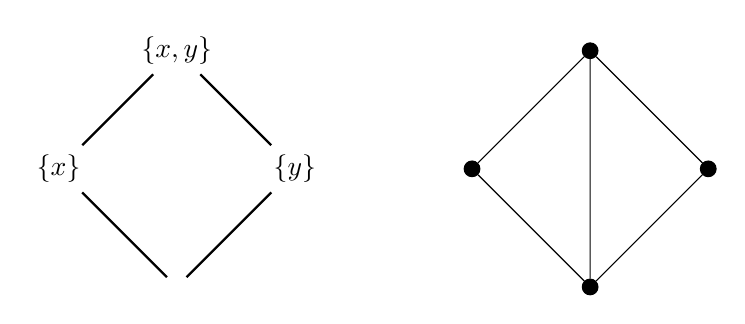
\begin{tikzpicture}[scale=1.5]

  % poset
  \draw (-1cm,0cm) node (v2) {$\{x\}$};
  \draw (1cm,0cm)  node (v3) { $\{y\}$ };
  \draw (0cm,-1cm) node (v4) {$\varnothing$};
  \draw (0cm,1cm)  node (v1) {$\{x,y\}$};

  \draw[thick]  (v1) edge (v2);
  \draw[thick]  (v3) edge (v1);
  \draw[thick]  (v3) edge (v4);
  \draw[thick]  (v2) edge (v4);

  % graph
  \node[draw,circle,inner sep=2pt,fill,label distance=1cm] (v1g) at (3.5,1) {};
  \node[draw,circle,inner sep=2pt,fill,label distance=1cm] (v2g) at (3.5,-1) {};
  \node[draw,circle,inner sep=2pt,fill,label distance=1cm] (v3g) at (4.5,0) {};
  \node[draw,circle,inner sep=2pt,fill,label distance=1cm] (v4g) at (2.5,0) {};
  \draw  (v1g) edge (v2g);
  \draw  (v1g) edge (v4g);
  \draw  (v4g) edge (v2g);
  \draw  (v1g) edge (v3g);
  \draw  (v3g) edge (v2g);

\end{tikzpicture}
\end{scaletikzpicturetowidth}

\caption{On the left, Hasse diagram of a poset of the power set of 2 elements ordered by inclusion.
On the right, the comparability graph of this poset.}
\label{fig:hasse}
\end{figure}

\subsubsection{Interval graphs}

An interval graph is a graph $G$ that is the intersection graph of a collection
of closed intervals in $\mathbb{R}$. If the length of each interval is unitary,
then $G$ is a unit interval graph (UIG).

\begin{theorem}
  $G$ is an interval graph if and only if every simple cycle of four or more
  points has a chord. \cite{FISHBURN1985135}
\end{theorem}

\begin{theorem}
  An interval graph is a unit interval graph if and only if it has no induced subgraph $K_{1,3}$ \cite{roberts1968representations}.
\end{theorem}

Another interesting class of interval graphs are mixed unit interval graphs, where each
interval can be closed, open, open-closed or closed-open. In this paper we will
denote those four classes like this:

$$\mathcal{I}^{++} = \{[x,y] : x,y \in \mathbb{R}, x\leq y\}$$
$$\mathcal{I}^{--} = \{(x,y) : x,y \in \mathbb{R}, x\leq y\}$$
$$\mathcal{I}^{+-} = \{[x,y) : x,y \in \mathbb{R}, x\leq y\}$$
$$\mathcal{I}^{-+} = \{(x,y] : x,y \in \mathbb{R}, x\leq y\}$$

$\mathcal{I}$ will be replaced by $\mathcal{U}$ when we are talking about unit
mixed interval graphs and their class is denoted MUIG.

\begin{theorem}
  The classes of the graphs $\mathcal{U}^{--}$, $\mathcal{U}^{++}$,
  $\mathcal{U}^{-+}$, $\mathcal{U}^{+-}$, and  $\mathcal{U}^{-+} \cup
  \mathcal{U}^{+-}$ are the same (equivalent for $\mathcal{I}$). \cite{DOURADO20123357}
\end{theorem}



\begin{figure}
\centering


\begin{scaletikzpicturetowidth}{\textwidth}
\begin{tikzpicture}[scale=1.5]

  \draw[{(-)}] (-1,-0.5) -- (0,-0.5);
  \draw[color=black] (-0.4845,-0.8507) node {$v_4$};
  \draw[{[-}] (0,-1.5) -- (1,-1.5);
  \draw[color=black] (0.5023,-1.3568) node {$v_3$};
  \draw[{-]}] (-2,-1.5) -- (-1,-1.5);
  \draw[color=black] (-0.4899,-0.3468) node {$v_2$};
  \draw[{[-]}] (-1,-1) -- (0,-1);
  \draw[color=black] (-1.4962,-1.3536) node {$v_1$};

  \node[draw,circle,inner sep=2pt,fill,label distance=1cm] (v1) at (-4,-0.25) {};
  \draw[color=black] (-4,0) node {$v_4$};
  \node[draw,circle,inner sep=2pt,fill,label distance=1cm] (v3) at (-4,-1.25) {};
  \draw[color=black] (-4,-1.5) node {$v_2$};
  \node[draw,circle,inner sep=2pt,fill,label distance=1cm] (v2) at (-5,-1.25) {};
  \draw[color=black] (-3,-1.5) node {$v_3$};
  \node[draw,circle,inner sep=2pt,fill,label distance=1cm] (v4) at (-3,-1.25) {};
  \draw[color=black] (-5,-1.5) node {$v_1$};
  \draw  (v1) edge (v2);
  \draw  (v1) edge (v3);
  \draw  (v1) edge (v4);

\end{tikzpicture}
\end{scaletikzpicturetowidth}

\caption{Representation of $K_{1,3}$ as a MUIG.}
\label{fig:muigK13}
\end{figure}

Unlike for UIG class, $K_{1,3}$ is a MUIG as seen in figure \ref{fig:muigK13}. Some
characterizations have been already found for these classes of graphs \cite{shuchatUnitMixedInterval2014a}
\cite{joosCharacterizationMixedUnit2013}.

\todo[inline]{Exploit these characterizations!! $\to$ explain them and use them to characterize UUIG.}

\subsubsection{Disks}

A disk graph $G$ is a graph that is an intersection graph of disks on the plane, when the size
of the disk is unitary, we talk about unit disk graphs. This class of graphs
is important for this thesis, as thin strip graphs are a sub-class of
unit disk graphs.

We will refer to the unit disk graph class as UDG and an example of a realization
can be found in the figure \ref{fig:udg}.

\paragraph{Induced forbidden subgraphs} The characterization of this class with respect to
its induced forbidden subgraphs has been studied \cite{atminasForbiddenInducedSubgraphs2016}.

\begin{theorem}[Atminas-Zamaraev]
  For every integer $k > 1$, $\overline{K_2 + C_{2k+1}}$ is a minimal induced subgraph.
\end{theorem}

\begin{theorem}[Atminas-Zamaraev]
  For every integer $k > 4$, $\overline{C_{2k}}$ is a minimal induced subgraph.
\end{theorem}

\begin{figure}
\centering

\begin{scaletikzpicturetowidth}{\textwidth}
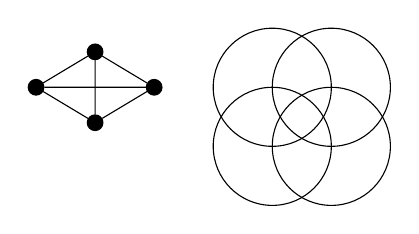
\begin{tikzpicture}[scale=1.5]

  \draw (-0.5,2.5) circle [radius=0.5];
  \draw (0,2.5) circle [radius=0.5];
  \draw (-0.5,2) circle [radius=0.5];
  \draw (0,2) circle [radius=0.5];


  \node[draw,circle,inner sep=2pt,fill,label distance=1cm] (v1) at (-2.5,2.5) {};

  \node[draw,circle,inner sep=2pt,fill,label distance=1cm] (v2) at (-2,2.2) {};
  \node[draw,circle,inner sep=2pt,fill,label distance=1cm] (v3) at (-2,2.8) {};
  \node[draw,circle,inner sep=2pt,fill,label distance=1cm] (v4) at (-1.5,2.5) {};

  \draw  (v3) edge (v2);
  \draw  (v4) edge (v1);
  \draw  (v3) edge (v1);
  \draw  (v4) edge (v2);
  \draw  (v3) edge (v4);
  \draw  (v1) edge (v2);

\end{tikzpicture}
\end{scaletikzpicturetowidth}

\caption{Realization of a UDG (Unit Disk Graph).}
\label{fig:udg}
\end{figure}
